%%%%%%%%%%%%%%%%%%%%%%%%%%%%%%%%%%%%%%%%%%%%%%%%%%%%%%%%%%%%%%%%%%%%%%%%%%%
%
% Plantilla para un artículo en LaTeX en español.
%
%%%%%%%%%%%%%%%%%%%%%%%%%%%%%%%%%%%%%%%%%%%%%%%%%%%%%%%%%%%%%%%%%%%%%%%%%%%

\documentclass[11pt,twocolumn,spanish]{article}

% Esto es para que el LaTeX sepa que el texto está en español:
\usepackage[spanish]{babel}

% Paquetes de la AMS:
\usepackage{amsmath, amsthm, amsfonts}


\usepackage[utf8]{inputenc}
\usepackage{amsmath}
\usepackage{amsfonts}
\usepackage[spanish]{babel}
\usepackage{latexsym}
\usepackage{euscript}
\usepackage{graphicx}
\usepackage{tdclock}
\usepackage{enumerate} 
\usepackage{float}
\usepackage{multirow, array} 
\usepackage[latin1]{inputenc}
\usepackage{caption}
\usepackage[dvips]{graphicx}

% tamaño de hoja
\oddsidemargin 0.05in
\textwidth 6.3in
\topmargin -0.5in
\headheight 0in
\textheight 9in 

% Teoremas
%--------------------------------------------------------------------------
\newtheorem{thm}{Teorema}[section]
\newtheorem{cor}[thm]{Corolario}
\newtheorem{lem}[thm]{Lema}
\newtheorem{prop}[thm]{Proposición}
\theoremstyle{definition}
\newtheorem{defn}[thm]{Definición}
\theoremstyle{remark}
\newtheorem{rem}[thm]{Observación}

% Atajos.
% Se pueden definir comandos nuevos para acortar cosas que se usan
% frecuentemente. Como ejemplo, aquí se definen la R y la Z dobles que
% suelen representar a los conjuntos de números reales y enteros.
%--------------------------------------------------------------------------

\def\RR{\mathbb{R}}
\def\ZZ{\mathbb{Z}}

% De la misma forma se pueden definir comandos con argumentos. Por
% ejemplo, aquí definimos un comando para escribir el valor absoluto
% de algo más fácilmente.
%--------------------------------------------------------------------------
\newcommand{\abs}[1]{\left\vert#1\right\vert}

% Operadores.
% Los operadores nuevos deben definirse como tales para que aparezcan
% correctamente. Como ejemplo definimos en jacobiano:
%--------------------------------------------------------------------------
\DeclareMathOperator{\Jac}{Jac}

%--------------------------------------------------------------------------
\title{Caos}
\author{Oscar De la Cruz Echeveste\\
  \small Dept. Plantillas y Editores\\
  \small E12345\\
  \small España
}

\begin{document}
\maketitle

\abstract{Esto es una plantilla simple para un artículo en \LaTeX.}

\section{Introducción}

Galileo Galilei, matemático y astrónomo italiano del siglo XVI y XVII, famoso por su icónica riña contra los miembros de la iglesia católica al tratar de mostrar como algunos cuerpos celeste no giraban alrededor de la tierra, como el mismo lo pudo observar en el movimiento de las lunas Jovianas. Atrevimientos como este y su carácter necio y egocéntrico lo llevaron a la excomunión y al arresto domiciliario por el resto de sus días. En el proceso en el que Galileo se adentro en la filosofía natural, observo como los cuerpos en movimiento evolucionaban a lo largo del tiempo y parecían obedecer ciertos patrones que eran predecibles al describirse en forma matemática. Tal fue su fascinación que dedico su vida a estudiar esta armonía que él encontraba en la naturaleza. “La matematica è la lingua in cui Dio ha scritto l'universo” es una de las frases que se le atribulen a Galileo y, aunque desconozco la veracidad de esta cita, es una de mis frases favoritas. Por una extraña razón la naturaleza puede caracterizarse por modelos matemáticos con los cuales podemos predecir la evolución o cambios en el sistema con una envidiable exactitud. En general, esta es la tarea a la que se adentra un físico. La matemática se vuelve la herramienta de trabajo más poderosa que da paz y tranquilidad en la certidumbre que caracteriza y predice la evolución de los sistemas. Pero la realidad es más complicada de lo que se espera. Ciertamente, la dinámica de muchos de los sistemas que se estudian no es tan sencilla de predecir. Uno se estos sistemas, y tal vez el de mayor antigüedad, es el problema de los tres cuerpos, él cual consta de tres objetos en movimiento afectados por la gravedad de cada uno. Tanto Newton (1642 - 1727) como otros matemáticos estudiaron este problema por los últimos siglos. Fue el matemático francés Henri Poincaré (1854 - 1912) quien demostró que no había una solución analítica para este problema y agrego que esto representaba la naturaleza del caos. 

Poincaré fue un pionero en el estudio del caos, un concepto que hasta hoy en día parece ser desconocido para muchos, temido por algunos y apasionado para otros pero sin duda un dolor de cabeza para todo aquel estudioso de esta área. Trabajar con el caos significa trabaja con sistemas dinámicos no lineales, es decir — 

Aquí va el texto.
\begin{equation}\label{eq:area}
  S = \pi r^2
\end{equation}
Uno puede referirse a ecuaciones así: ver ecuación (\ref{eq:area}).
También se pueden mencionar secciones de la misma forma: ver sección
\ref{sec:nada}. O citar algo de la bibliografía: \cite{Cd94}.

\section{Mapeo}\label{sec:nada}

En matemáticas un mapeo, aplicación o  función es una regla que asocia valores de algún conjunto que llamaremos \textit{conjunto objeto} \textbf{A} a un \textit{conjunto objetivo} \textbf{B}. Podemos representar esto de manera gráfica como:

\begin{equation*}
\begin{split}
&f:  A \longrightarrow B \\
&a  \mapsto f(a) = b  
\end{split}
\end{equation}

Donde f es la regla de asociación entre los valores (a) del conjunto A  a los valores (b) del conjunto B. Un ejemplo sencillo es una función $f:  IR \longrightarrow IR $ tal que $x \mapsto f(x) = 2x$ donde la función $f$ relacionas los elementos del conjunto de los números reales con los elementos de un conjunto igual de tal forma que cada elemento del conjunto objetivo es el doble de un sólo elemento del conjunto objeto. 


\begin{figure}[H]
\centering
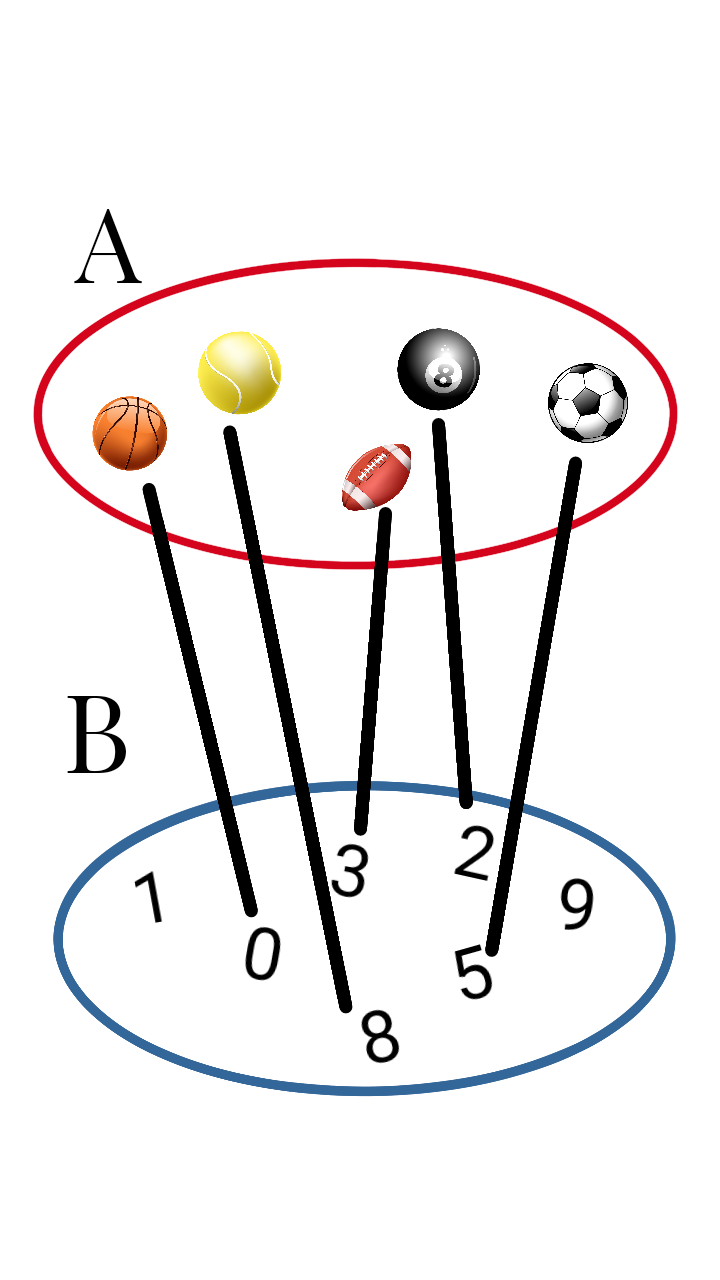
\includegraphics[width=3cm]{figura_1}
\caption*{\textbf{Figura 2.1}: Representación gráfica de un mapeo de conjuntos de pelotas deportivas al conjunto de números naturales $\mathbb{N}$ }
\label{etiqueta}
\end{figure}
\end{enumerate}

\subsubsection{Subsubsection}\label{sec:nada2}

Más texto.

% Bibliografía.
%-----------------------------------------------------------------
\begin{thebibliography}{99}

\bibitem{Cd94} Autor, \emph{Título}, Revista/Editor, (año)

\end{thebibliography}

\end{document}